\begin{center}
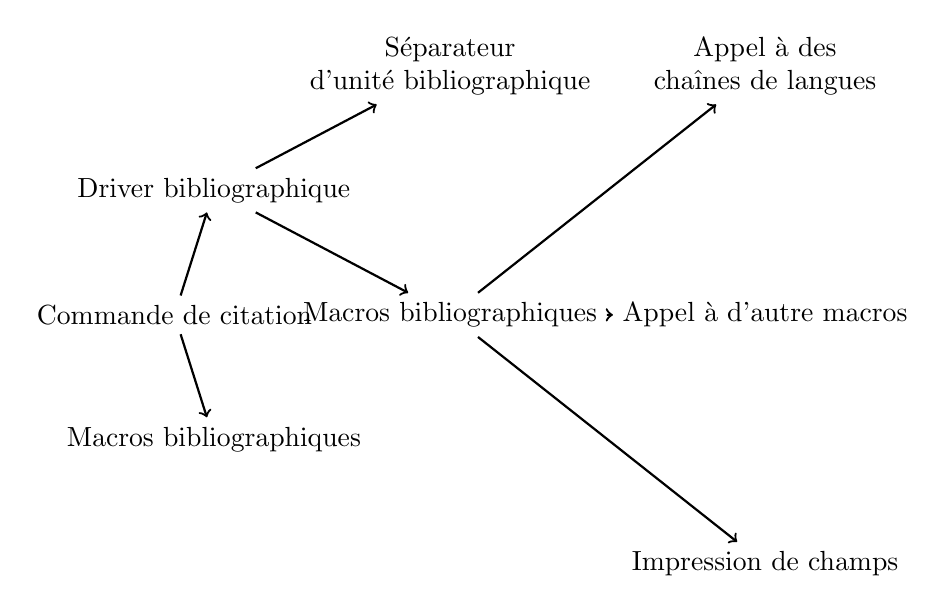
\begin{tikzpicture}[edge from parent path={[->,thick]
      (\tikzparentnode) -- (\tikzchildnode)},grow=right,level 1/.style={sibling distance=9em,level distance=.5cm},level 2/.style={sibling distance=9em,level distance=3cm},level 3/.style={sibling distance=9em,level distance=4cm},
	every node/.style={align=center}]
	\node {Commande de citation} 
		child { node {Macros bibliographiques}}
		child { node {Driver bibliographique}
			child { node {Macros bibliographiques}
			 	child {
					node{Impression de champs}
					}
			 	child {
					node{Appel à d'autre macros}
					}
				child {
					node{Appel à des \\ chaînes de langues}
					}
				}
			child { node {Séparateur\\ d'unité bibliographique}}
			}	
	;		
\end{tikzpicture}
\end{center}